\documentclass{ximera}

\newcommand{\RR}{\mathbb R}
\renewcommand{\d}{\,d}
\newcommand{\dd}[2][]{\frac{d #1}{d #2}}
\renewcommand{\l}{\ell}
\newcommand{\ddx}{\frac{d}{dx}}
\newcommand{\dfn}{\textbf}
\newcommand{\eval}[1]{\bigg[ #1 \bigg]}


\outcome{Solve basic related rates word problems.}
\outcome{Understand the process of solving related rates problems.}
\outcome{Calculate derivatives of expressions with multiple variables implicitly.}

\title[Dig-In:]{More than one rate}

\begin{document}
\begin{abstract}
  Here we work abstract related rates problems.
\end{abstract}
\maketitle


Suppose we have two variables $x$ and $y$ which are both changing with
respect to time.  A \textit{related rates} problem is a problem where
we know one rate at a given instant, and wish to find the other.

Here the chain rule is key: If $y$ is written in terms of $x$, and we
are given $\dd[x]{t}$, then it is easy to find $\dd[y]{t}$ using the
chain rule:
\[
\dd[y]{t}=y'(x(t))\cdot x'(t).
\]
In many cases, particularly the interesting ones, our functions will
be related in some other way. Nevertheless, in each case we'll use the
power of the chain rule to help us find the desired rate. In this
section, we will work several abstract examples, so we can emphasize
the mathematical concepts involved. In each of the examples below, we
will follow essentially the same plan of attack:

\begin{description}
\item[\textbf{Draw a picture.}] If possible, draw a schematic picture
  with all the relevant information.
\item[\textbf{Find equations.}] We want equations that relate all
  relevant functions.
\item[\textbf{Differentiate the equations.}] Here we will often use
  implicit differentiation.
\item[\textbf{Evaluate.}] Evaluate
  each equation at the  relevant moment. 
    \item[\textbf{Solve.}] Solve for the relevant
  rate at the relevant moment.

\end{description}


\section{Formulas}

One way to combine several functions is with a known formula.

\begin{example}
  Imagine an expanding circle. If we know that the perimeter is
  expanding at a rate of $4$ m/s, what rate is the area changing
  when the radius is $3$ meters?
  \begin{explanation}
    To start, we \textbf{draw a picture}.
    \begin{image}
      \begin{tikzpicture}
        \draw [penColor, very thick] (0,0) circle [radius=2];
        \draw [penColor] (0,0) -- (2,0);
        \node [below,penColor] at (1,0) {$r=3$ m};
        \node [penColor,left] at (-1.5,1.42) {$\dfrac{d}{dt}P(t) = 4$ m/s};
        \node [penColor, right] at (1.5,-1.42) {$A = \pi\cdot r^2$};
      \end{tikzpicture}
    \end{image}
    We must \textbf{find equations} that combine relevant
    functions. Here we use the common formulas for perimeter and area
    \[
    P = \answer[given]{2\cdot \pi \cdot r}
    \qquad\text{and}\qquad
    A = \answer[given]{\pi \cdot r^2}.
    \]
    Next we imagine that $A$, $r$, and $P$ are functions of time
    \[
    P(t) = 2\cdot \pi \cdot r(t)
    \qquad\text{and}\qquad
    A(t) = \pi \cdot r(t)^2.
    \]
    and we \textbf{differentiate the equations} using implicit
    differentiation, treating all functions as functions of $t$
    \[
    \dfrac{d}{dt}P(t) = 2\cdot \pi\cdot  \dfrac{d}{dt}r(t)
    \qquad\text{and}\qquad
     \dfrac{d}{dt}A(t) = 2\cdot \pi\cdot r(t) \cdot  \dfrac{d}{dt}r(t).
    \]
    Now we \textbf{evaluate} all the quantities at the moment when $r=3$.
    
     We know  that at that moment $\Bigl[ \dfrac{d}{dt}P(t)\Bigr]_{r=3} =
    \answer[given]{4}$ and that $r = \answer[given]{3}$. Hence our
    equations become
    \[
    4 = 2\cdot \pi\cdot \Bigl[\dfrac{d}{dt}r(t)\Bigr]_{r=3}
    \qquad\text{and}\qquad
   \Bigl[ \dfrac{d}{dt}A(t)\Bigr]_{r=3} = 2\cdot \pi\cdot 3 \cdot \Bigl[\dfrac{d}{dt}r(t)  \Bigl]_{r=3}.
    \]
    We see that
    \begin{align*}
       4 &= 2\cdot \pi\cdot \Bigl[\dfrac{d}{dt}r(t)\Bigr]_{r=3}\\
      2/\pi &=  \Bigl[\dfrac{d}{dt}r(t)\Bigr]_{r=3}.
    \end{align*}
    
   Now we \textbf{solve} for the rate of $A$ at the moment when $r=3$.
   
    \begin{align*}
     \Bigl[ \dfrac{d}{dt}A(t)\Bigr]_{r=3} &= 2\cdot \pi\cdot 3 \cdot 2/\pi\\
      &=\answer[given]{12}.
    \end{align*}
    Hence the area is expanding at a rate of $12$ m/s at the moment when the radius is 3 meters.
  \end{explanation}
\end{example}


%%BADBAD
%% There are a number of common formulas that arise in related rates
%% problems.
%%
%% It might be nice to add a little list of common area/volume formulas.



\section{Right triangles}

A common way to combine functions is through facts related to right
triangles.


\begin{example}
  Imagine an expanding right triangle. If one leg has a fixed length
  of $3$ m, one leg is increasing with a rate of $2$ m/s, and the
  hypotenuse is expanding to accommodate the expanding leg, at what
  rate is the hypotenuse expanding when both legs are $3$ m long?
  \begin{explanation}
    To start, we \textbf{draw a picture}.
    \begin{image}
      \begin{tikzpicture}
        \coordinate (A) at (0,2);
        \coordinate (B) at (0,5);
        \coordinate (C) at (6.5,2);
        \tkzMarkRightAngle(C,A,B)
        \tkzDefMidPoint(A,B) \tkzGetPoint{a}
        \tkzDefMidPoint(A,C) \tkzGetPoint{b}
        \tkzDefMidPoint(B,C) \tkzGetPoint{c}
        \draw (A)--(B)--(C)--cycle;
        \tkzLabelPoints[above](c)
        \tkzLabelPoints[above](b)
        %\tkzLabelPoints[left](a)
        \node [left] at (a) {$a = 3$};
        \node [below] at (b) {$b'(t) = 2$};
      \end{tikzpicture}
    \end{image}

    We must \textbf{find equations} that combine relevant
    functions. Here we use the Pythagorean Theorem.
    \[
    c^2 = a^2 + b^2
    \]
    Imagining $c$ and $b$ as being functions of time
    \[
    c(t)^2 = a^2 + b(t)^2
    \]
    we are now able to \textbf{differentiate the equation} using
    implicit differentiation, treating all functions as functions of
    $t$, note $a$ is constant,
    \[
    2\cdot c(t)\cdot \dfrac{d}{dt}c(t) = 2\cdot b(t)\cdot \dfrac{d}{dt}b(t).
    \]
    Now we \textbf{evaluate}. We
    know that $\Bigl[\dfrac{d}{dt}b(t)\Bigr]_{b=3} = 2$ and that $b = 3$
    \[
    2\cdot [c(t)]_{b=3}\cdot \Bigl[\dfrac{d}{dt}c(t)\Bigr]_{b=3} = \answer[given]{12}
    \]
    However, we still need to know $[c(t)]_{b=3}$, the length of the hypotenuse at the moment when $b=3$. Here we use
    the Pythagorean Theorem,
    \begin{align*}
    \Bigl([c(t)]_{b=3}\Bigr)^2 &= 3^2 + 3^2\\
    &=\answer[given]{18},
    \end{align*}
    and so we see that $[c(t)]_{b=3} = 3\sqrt{2}$. \\
    And we \textbf{solve} for the rate.\\
    \begin{align*}
      6\sqrt{2}\cdot \Bigl[\dfrac{d}{dt}c(t)\Bigr]_{b=3} &= 12 \\     
      \Bigl[\dfrac{d}{dt}c(t)\Bigr]_{b=3} &= \sqrt{2}.
    \end{align*}
    Hence $c(t)$ is growing at a rate of $\answer[given]{\sqrt{2}}$ m/s when both legs are $3m$ long.
  \end{explanation}
\end{example}


\section{Angular rates}


We can also investigate problems involving angular rates.

\begin{example}
  Imagine an expanding right triangle. If one leg has a fixed length
  of $3$ m, one leg is increasing with a rate of $2$ m/s, and the
  hypotenuse is expanding to accommodate the expanding leg, at what
  rate is the angle opposite the fixed leg changing when both legs
  are $3$ m long?
  \begin{explanation}
    To start, we \textbf{draw a picture}.
    \begin{image}
      \begin{tikzpicture}
        \coordinate (A) at (0,2);
        \coordinate (B) at (0,5);
        \coordinate (C) at (6.5,2);
        \tkzMarkRightAngle(C,A,B)
        \tkzMarkAngle[size=1.2cm,thin](B,C,A)
        \tkzLabelAngle[pos = 1](B,C,A){$\theta$}
        \tkzDefMidPoint(A,B) \tkzGetPoint{a}
        \tkzDefMidPoint(A,C) \tkzGetPoint{b}
        \tkzDefMidPoint(B,C) \tkzGetPoint{c}
        \draw (A)--(B)--(C)--cycle;
        \tkzLabelPoints[above](c)
        \tkzLabelPoints[above](b)
        %\tkzLabelPoints[left](a)
        \node [left] at (a) {$a = 3$};
        \node [below] at (b) {$b'(t) = 2$};
      \end{tikzpicture}
    \end{image} 

    We must \textbf{find equations} that combines relevant
    functions. Here we note that
    \[
    \tan(\theta) = \answer[given]{\frac{a}{b}}
    \]
    Imagining $\theta$ and $b$ as being functions of time
    \[
    \tan(\theta(t)) = \frac{a}{b(t)}
    \]
    we are now able to \textbf{differentiate the equation} using
    implicit differentiation, treating all functions as functions of
    $t$, note $a$ is constant,
    \[
    \sec^2(\theta(t))\theta'(t) = \frac{-a\cdot b'(t)}{b(t)^2}.
    \]
    Now we \textbf{evaluate}.  We
    know that $a=3$, $b'(t) = 2$, and that $b = 3$
    \begin{align*}
    \Bigl[\sec^2(\theta(t))\Bigr]_{b=3}\cdot \Bigl[\dfrac{d}{dt}\theta(t)\Bigr]_{b=3} &= \frac{-3\cdot 2}{3^2}\\
    &= \frac{-6}{9}\\
    &= \frac{-2}{3}.
    \end{align*}
    However, we still need to know $ \Bigl[\sec^2(\theta(t))\Bigr]_{b=3}$. Here we use the
    Pythagorean Theorem,
    \begin{align*}
    [c^2(t)]_{b=3} &= 3^2 + 3^2\\
    &=\answer[given]{18},
    \end{align*}
    and so we see that $[c(t)]_{b=3} = 3\sqrt{2}$. Now
    \begin{align*}
     \Bigl[\sec^2(\theta(t))\Bigr]_{b=3} &= \frac{\mathrm{hypotenuse}^2}{\mathrm{adjacent}^2}\\
      &= \frac{\left(3\sqrt{2}\right)^2}{3^2}\\
      &= \answer[given]{2}.
    \end{align*}
   Now we \textbf{solve}.
    \begin{align*}
    \Bigl[\sec^2(\theta(t))\Bigr]_{b=3}\cdot \Bigl[\dfrac{d}{dt}\theta(t)\Bigr]_{b=3}  &= \frac{-2}{3}\\
      2\cdot \Bigl[\dfrac{d}{dt}\theta(t)\Bigr]_{b=3}  &= \frac{-2}{3}\\
     \Bigl[\dfrac{d}{dt}\theta(t)\Bigr]_{b=3} &= \frac{-1}{3}.
    \end{align*}
    So when $a=b=3$, the angle is changing at $\answer[given]{-1/3}$
    radians per second.
  \end{explanation}
\end{example}



\section{Similar triangles}

Finally, facts about similar triangles are often useful when solving
related rates problems.

\begin{example}
  Imagine two right triangles that share an angle:
  \begin{image}
    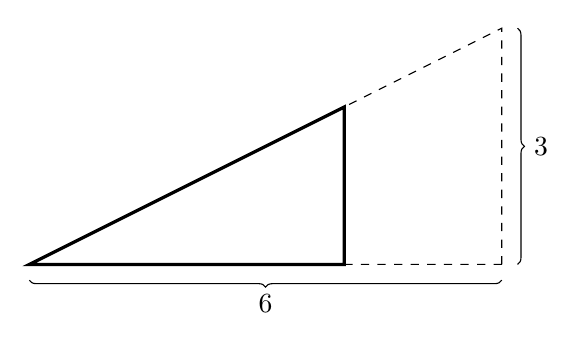
\begin{tikzpicture}
      \coordinate (A) at (6,2);
      \coordinate (B) at (6,5);
      \coordinate (C) at (0,2);
      \coordinate (D) at (4,2);
      \coordinate (E) at (4,4);
      \tkzMarkRightAngle(C,A,B)
      \tkzMarkRightAngle(C,D,E)
      \tkzDefMidPoint(A,B) \tkzGetPoint{a}
      \tkzDefMidPoint(A,C) \tkzGetPoint{b}
      \tkzDefMidPoint(D,C) \tkzGetPoint{x}
      \draw[decoration={brace,mirror,raise=.2cm},decorate,thin] (0,2)--(6,2);
      \draw[decoration={brace,mirror,raise=.2cm},decorate,thin] (6,2)--(6,5);
      \draw[dashed] (A)--(B)--(C)--cycle;
      \draw[very thick] (D)--(E)--(C)--cycle;
      \tkzLabelPoints[above](x)
      \node at (3,2-.5) {$6$};
      \node at (6+.5,3.5) {$3$};
    \end{tikzpicture}
  \end{image}
  If $x$ is growing from the vertex with a rate of $3$ m/s, what rate
  is the area of the smaller triangle changing when $x = 5$m?
  \begin{explanation}
    Despite the fact that a nice picture is given, we should start as
    we always do and \textbf{draw a picture}. Note, we've added
    information to the picture:
    \begin{image}
      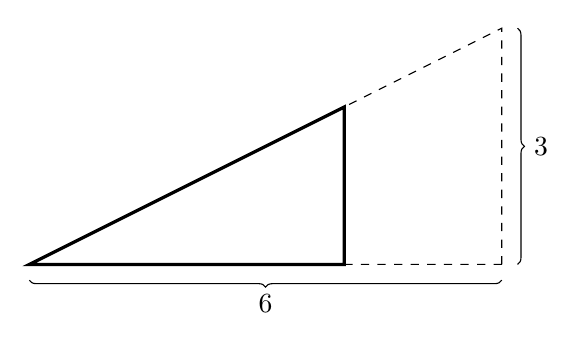
\begin{tikzpicture}
        \coordinate (A) at (6,2);
        \coordinate (B) at (6,5);
        \coordinate (C) at (0,2);
        \coordinate (D) at (4,2);
        \coordinate (E) at (4,4);
        \tkzMarkRightAngle(C,A,B)
        \tkzMarkRightAngle(C,D,E)
      \tkzDefMidPoint(A,B) \tkzGetPoint{a}
      \tkzDefMidPoint(A,C) \tkzGetPoint{b}
      \tkzDefMidPoint(D,C) \tkzGetPoint{x}
      \tkzDefMidPoint(D,E) \tkzGetPoint{h}
      \draw[decoration={brace,mirror,raise=.2cm},decorate,thin] (0,2)--(6,2);
      \draw[decoration={brace,mirror,raise=.2cm},decorate,thin] (6,2)--(6,5);
      \draw[dashed] (A)--(B)--(C)--cycle;
      \draw[very thick] (D)--(E)--(C)--cycle;
      \tkzLabelPoints[above](x)
      \tkzLabelPoints[right](h)
      \node at (3,2-.5) {$6$};
      \node at (6+.5,3.5) {$3$};
    \end{tikzpicture}
  \end{image}


    We must \textbf{find equations} that combine relevant
    functions. In this case there are two. The first is the formula
    for the area of a triangle:
    \[
    A = \answer[given]{(1/2) \cdot x \cdot h}
    \]
    The second uses the fact that the larger triangle is similar to
    the smaller triangle, meaning that the proportions of the sides
    are the same,
    \[
    \frac{x}{h} = \answer[given]{\frac{6}{3}}\qquad\text{so}\qquad x =
    \answer[given]{2}\cdot h
    \]
    Imagining $A$, $x$, and $h$ as functions of time we may write
    \[
    A(t) = (1/2) \cdot x(t) \cdot h(t) \qquad\text{and}\qquad x(t) =
    2\cdot h(t).
    \]
    We are now able to \textbf{differentiate the equations} using
    implicit differentiation, treating all functions as functions of
    $t$,
    \begin{align*}
    \dfrac{d}{dt}A(t) &= (1/2) \cdot\dfrac{d}{dt}x(t) \cdot h(t) +  (1/2) \cdot x(t) \cdot \dfrac{d}{dt}h(t),\\
     \dfrac{d}{dt}x(t) &= 2\cdot\dfrac{d}{dt}h(t)
    \end{align*}
    Now we \textbf{evaluate} at the moment when $x=5$m.
   We know that $x'(t) = 3$. Since
    \[
    5 = 2\cdot [h(t)]_{x=5}\qquad\text{and}\qquad 3= 2\cdot \Bigl[\dfrac{d}{dt}h(t)\Bigr]_{x=5}
    \]
    we see that $ [h(t)]_{x=5} = 5/2$ and $ \Bigl[\dfrac{d}{dt}h(t)\Bigr]_{x=5} = 3/2$. \\
    Now we \textbf{solve} for the rate.
    \begin{align*}
    \Bigl[\dfrac{d}{dt}A(t)\Bigr]_{x=5}  &= (1/2) \cdot 3 \cdot (5/2) + (1/2) \cdot 5 \cdot (3/2)\\
      &= 15/4 + 15/4\\
      &= \answer[given]{15/2}.
    \end{align*}
    Hence the area is changing at a rate of $15/2$ $\text{m}^2/\text{s}$ when $x=5$m.
    
  \end{explanation}
\end{example}
\end{document}
